\section{Pr�sentation du sujet}

\subsection{Le sujet}
\begin{frame}{Le sujet}
    \begin{block}{Probl�matique}
        \begin{itemize}
            \item Mod�lisation graphique : SysML
            \item V�rification de l'assemblage de blocs
            \item N�cessit� d'un langage formel

        \end{itemize}

    \end{block}

\end{frame}

%

\subsection{SysML}
\begin{frame}{Mod�lisation de syst�mes}
	\centering
	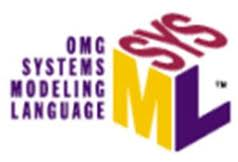
\includegraphics[scale=0.5]{./images/sysml.jpg}

    \begin{block}{SysML}
        \begin{itemize}
        	\item System Modeling Language
            \item Langage de mod�lisation graphique
            \item Bas� sur UML
            \item Adapt� � l'Ing�nierie Syst�me (syst�mes complexes h�t�rog�nes)

        \end{itemize}

    \end{block}

\end{frame}

\begin{frame}{Points communs et divergences avec UML}
    \centering
    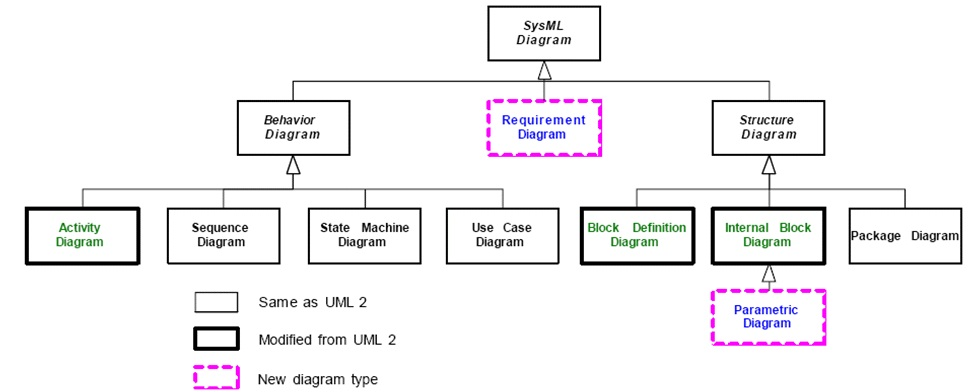
\includegraphics[scale=0.45]{./images/image5.jpg}

\end{frame}

%

\subsection{Automates d'interface}
\begin{frame}{Automates d'interface}
    \centering
    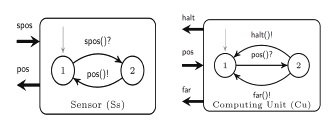
\includegraphics[scale=0.9]{./images/exempleAutomateInterface.jpg}
    \begin{block}{D�finition}
        \begin{itemize}
            \item Introduit par Alfaro et Henzinger
            \item Mod�lise les interface des composants
            \item Description des actions internes/entr�e/sortie

        \end{itemize}

    \end{block}

\end{frame}

%

\subsection{Vue globale du projet}
\begin{frame}{\'Etapes du projet}
    \centering
    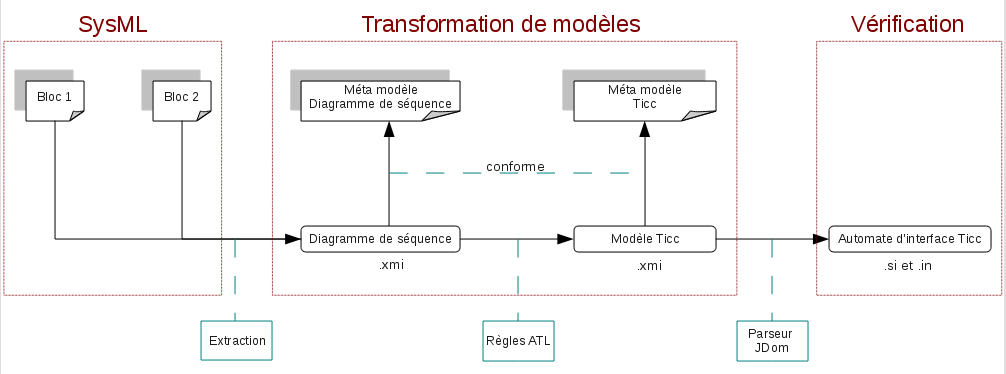
\includegraphics[scale=0.45]{./images/vueEnsemble.png}

\end{frame}



